\documentclass[hidelinks,12pt]{article}

\usepackage[brazil]{babel}
\usepackage[utf8]{inputenc}
\usepackage{amsmath}
\usepackage{amsfonts}
\usepackage{amssymb}
\usepackage{indentfirst}
\usepackage{color}
\usepackage{mathrsfs}
\usepackage{pgfplots}
\usepackage{hyperref}
\usepackage{fancyhdr}
\usepackage[export]{adjustbox}
\newcommand{\icon}[1]{\includegraphics[height=12pt]{#1}}

\fancypagestyle{plain}{%
	\fancyfoot{}%
	\fancyhead{}%
}
\fancyhead{}
\fancyhead[L]{\leftmark}
\fancyfoot{}
\fancyfoot[L]{{\footnotesize  COMPPET - Programa de Educação Tutorial}}
\fancyfoot[C]{\hspace{3.0cm}\thepage}
\fancyfoot[R]{{\footnotesize Curso de Inclusão Digital}}
\begin{document}
\pagestyle{fancy}
	
\tableofcontents
{\let\thefootnote\relax\footnotetext{* \textit{COMPPET - UFU, Universidade Federal de Uberlândia, Minas Gerais, Brasil}}}

{\let\thefootnote\relax\footnotetext{* \textit{PETMEC - UFU, Universidade Federal de Uberlândia, Minas Gerais, Brasil}}}

\newpage

\section{Introdução}
\paragraph{} Este material foi desenvolvido por alunos do PET-Computação, PET-Eng. Civil, PET-Eng. Mecânica da UFU - Universidade Federal de Uberlândia e visa prioritariamente ajudar aqueles que tiveram pouco/nenhum contato com o computador e o nicho o qual ele
			está inserido. Nos primeiros capítulos você aprenderá tarefas simples, como ligar e desligar o computador,utilizar o sistema operacional (Windows 7), depois mostraremos o tão famoso editor de texto Word, por fim um capitulo dedicado inteiramente à Internet, o que é, e como usá-la.
\paragraph{} Ao final do curso você será capaz de entender como um computador funciona e como usá-lo, contudo o mais importante
			é aprender a como buscar o que você deseja, pois mesmo se este curso durasse 6 meses não seriamos capazes 
			de ensinar tudo que é possível de se realizar com um computador, espero que goste e qualquer sugestão é sempre bem vinda.\textbf{Enfim chega de papo e vamos ao que realmente interessa!!!}

\section{Ligando e Desligando o Computador}
\subsection{Ligando o Computador} 

\paragraph{} Para ligar o computador, devemos seguir os seguintes passos: \\
\begin{itemize}
	
	\item Verificar os cabos de energia do computador;
	
	\item Verificar se a voltagem está correta (110 volts ou 220 volts);
	
	\item Verificar se existe um estabilizador \href{Fig:estabilizador} de voltagem, e se existir, verificar a voltagem da 
	dele (110 v ou 220 v). Essa voltagem deve ser compatível com a voltagem utilizada na sua casa, ou no trabalho;
	
	\item Quando todos os cabos estiverem conectados, ligar o estabilizador. Ele possui um botão Liga/Desliga de acesso e identificação simples;

	\item Ligar o PC através do botão Liga/Desliga, localizado no gabinete;
	
	\item Aguardar os procedimentos de inicialização do computador; 
	
	\item Informar senha e nome do usuário, caso existam e quando for solicitado.


\end{itemize}

\subsection{Desligando o Computador}
\paragraph{} O procedimento de desligar o computador é muito importante para preservar o equipamento e as informações armazenadas nele, portanto, é importantíssimo acostumar-se a seguir o procedimento de desligar:\\

\begin{itemize}
	\item Clicar no botão Iniciar;
	
	\item Clicar na opção Desligar; 
	
	\item Esperar o computador desligar automaticamente; 
	
	\item Desligar o estabilizador através do botão Liga/Desliga do estabilizador.
\end{itemize}

\begin{figure}[!hb]
	\centering	
	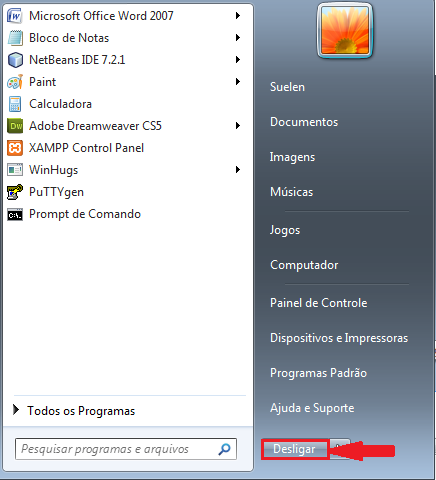
\includegraphics{Figures/desligando.png}
	\caption{Desligando o Computador}
	\label{fig:desligando}
\end{figure}

\newpage

\section{O windows 7}
\subsection{Área de Trabalho (Desktop)}

O Windows é o sistema operacional criado pela Microsoft Corporation® que tem como principal característica o uso de janelas para facilitar a utilização dos diversos aplicativos existentes no sistema. Antes do conceito de janelas, os sistemas operacionais eram utilizados em modo de texto. Ainda existem sistemas que se utilizam desse recurso, como é o caso de algumas versões do Linux.

No meio computacional, uma área de trabalho consiste de um ambiente gráfico adequado às necessidades de cada usuário. A área de trabalho permite a colocação de ícones dos programas mais utilizados, facilitando a vida do usuário.\\

\begin{figure}[!hb]
	\centering
	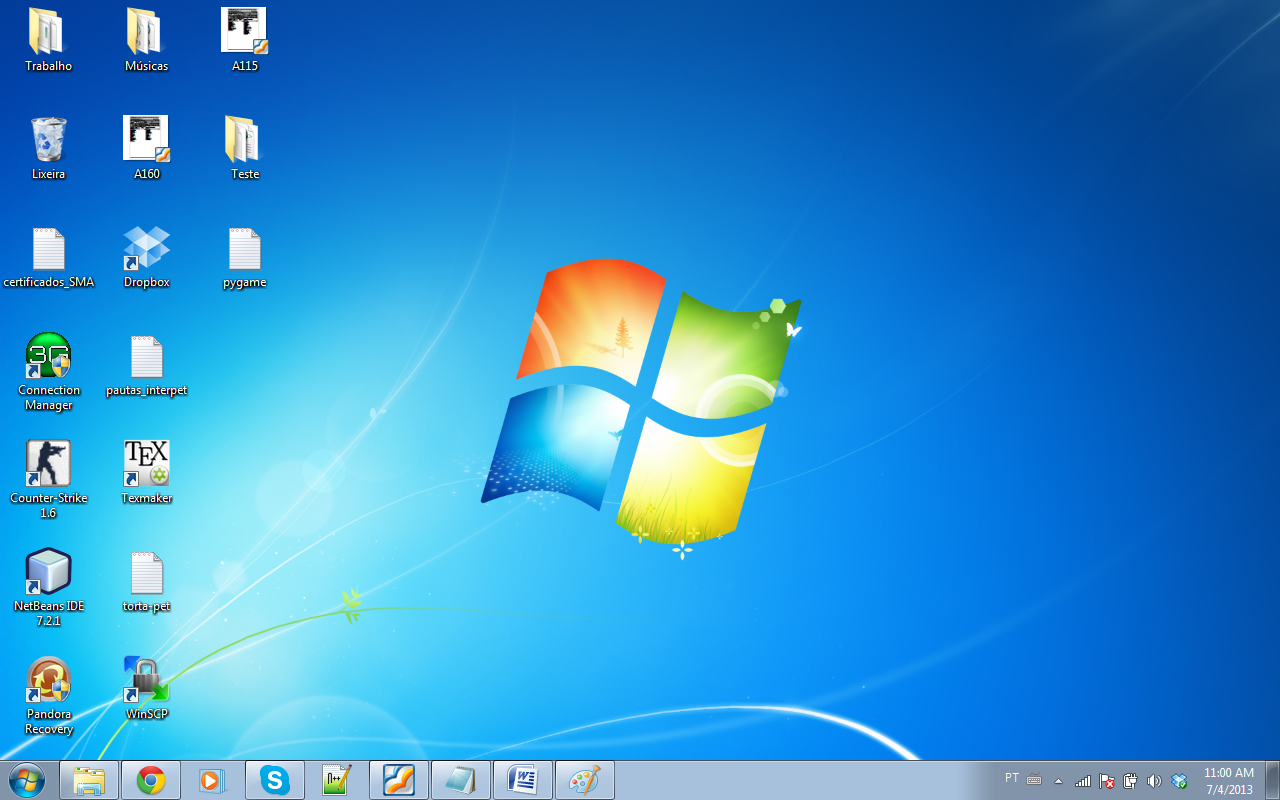
\includegraphics[scale=0.3]{Figures/desktop}
	\caption{Desktop}
	\label{fig:desktop}
\end{figure}


\subsection{Ícones}
	Os ícones na área de trabalho servem de atalhos para os programas mais utilizados.	
	Organizar os ícones da área de trabalho é uma tarefa semelhante a organizar as janelas. Em uma parte vazia do Desktop, clique no botão direito do mouse e selecione a opção: 

	Classificar por $->$ Nome
	
	 \hspace{3.6cm}Tamanho
	 
	 \hspace{3.6cm}Tipo de item
	 
	 \hspace{3.6cm}Data de modificação.
	
	 Existe uma outra opção chamada Exibir. Clicando nela com o botão esquerdo do mouse você pode Organizar ícones automaticamente. Uma outra opção é soltar o ícone em qualquer parte da área de trabalho.
	
	
	\begin{figure}[!htbp]
		\centering
		\begin{minipage}[b]{0.45\textwidth}
			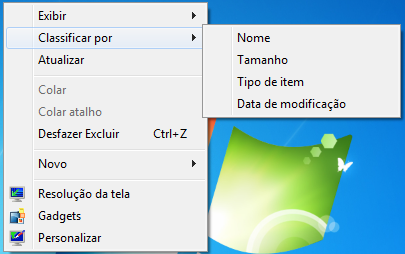
\includegraphics[width=\textwidth]{Figures/icone1}
			\caption{Classificar por}
			\label{fig:classificar por}
		\end{minipage}
		\hfill
		\begin{minipage}[b]{0.45\textwidth}
			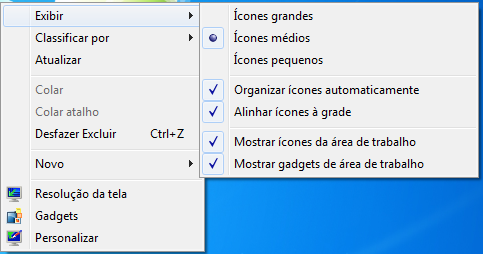
\includegraphics[width=\textwidth]{Figures/icone2}
			\caption{Exibir}
			\label{fig:exibir}
		\end{minipage}
	\end{figure}

\subsection{Barra de Tarefas}

	É uma barra de ferramentas gráficas usada para controlar a execução dos programas dispostos em janelas, classificando-as como ativa ou inativa. Tem como principal componente o botão iniciar.
	
	É subdividida em:
	
\begin{itemize}
	\item Menu Iniciar – nele estão organizados todos os programas do computador para um acesso imediato;

	\item Barra de Inicialização Rápida – podem ser colocados nesta área os programas mais utilizados pelo usuário;

	\item Janela Ativa ou Inativa – nesta área aparecem todas as janelas que estão ativas ou inativas (os programas que estão em execução são mostrados);

	\item Área de Notificação – os programas que estão sendo controlados pelo sistema aparecem nesta área, inclusive o relógio.
	
\end{itemize}
	
		\begin{figure}[!hb]
			%\centering
			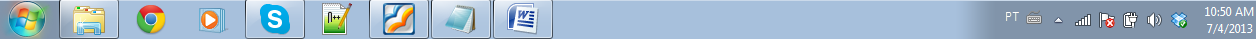
\includegraphics[width=1\textwidth,left]{Figures/menuiniciar}
			\label{fig:menu iniciar}
		
		\end{figure}	
	  {\vspace{-0.8cm}\hspace{-0.6cm}\huge{$\Downarrow$}}     {\vspace{-0.8cm}\hspace{3.6cm}\huge{$\Downarrow$}}
	  {\vspace{-0.8cm}\hspace{7.6cm}\huge{$\Downarrow$}}\\
	  \bigskip
	  
	  \vspace{1cm}
	  \hspace{-0.6cm}{\small Iniciar } \hspace{1cm}{\tiny Barra de Inicialização Rápida e Janelas Ativas e Inativas}
	  \hspace{1.2cm}{\small Área de Notificação}
	  \newpage
  
  \subsection{Relógio/Calendário}
	
	O relógio está localizado na extrema direita da barra de tarefas. Para fazer a visualização da data, basta clicar em cima da hora. Para fazer correção de hora e/ou data, basta clicar em {\bf Alterar configurações de data e hora}. 
	
	\begin{figure}[!hb]
		\centering
		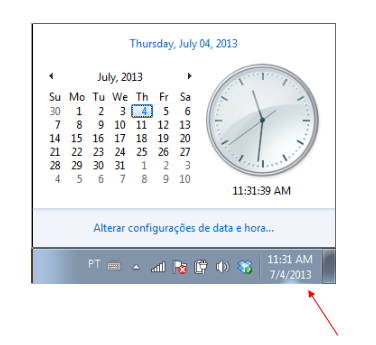
\includegraphics[scale=0.9]{Figures/relogio}
		\caption{Relógio do Windows 7}
		\label{fig:relogio}
		
	\end{figure}
	
	Após serem feitas as modificações de data e hora deve-se clicar no botão {\bf OK} para que as atualizações sejam salvas
	
	\begin{figure}[!h]
		\centering
		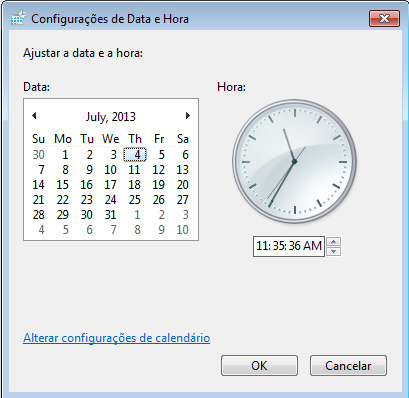
\includegraphics[scale=0.9]{Figures/relogio2}
		\caption{Calendário do Windows 7}
		\label{fig:calendario}
		
	\end{figure}
	
	\newpage
	\subsection{Menu Iniciar}
	
	Através do menu Iniciar podemos acessar os diversos recursos disponíveis em nosso computador. Nele estão contidos todos os programas instalados no computador, diversas ferramentas de manutenção do sistema e ferramentas úteis como a calculadora, bloco de notas e o Google Chrome \footnote{O naveggador padrão é o Internet Explorer, no entanto, o Chrome apresenta melhor desempenho.} que é o programa de navegação na internet . Ao se clicar neste, abrirá no computador uma janela semelhante a da figura abaixo:
	
	
	\begin{figure}[!h]
		\centering
		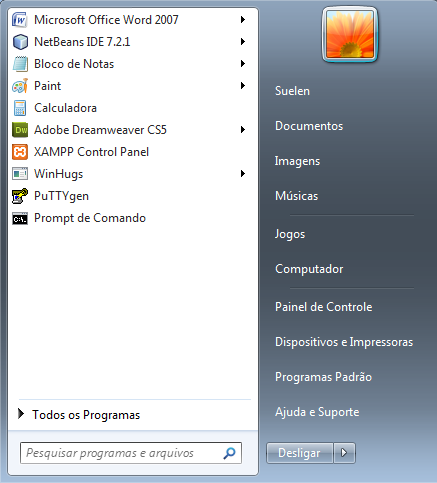
\includegraphics[scale=0.9]{Figures/iniciar}
		\caption{Iniciar}
		\label{fig:iniciar}
		
	\end{figure}
	\newpage
	\begin{itemize}
	\item Na coluna da esquerda, fica a lista dos programas usados mais recentemente.

	\item Todos os programas – Nele você encontra os ícones de todos os programas instalados assim como as ferramentas de administração do sistema.
	
	\item Documentos – Aqui podem ser guardados todos os documentos produzidos no computador.
	
	\item Imagens – É uma pasta para armazenagem de imagens.
	
	\item Músicas – É uma pasta que contém ou podem ser armazenados diversos formatos de áudio.
	
	\item Jogos – Aqui encontra-se todos os jogos disponíveis do computador.
	
	\item Computador – Aqui você pode ter acesso às pastas do sistema operacional.
	
	\item Painel de Controle – Contém opções de configuração do computador.
	
	\item Dispositivos e Impressoras – Aqui se encontram as impressoras e aparelhos de fax instalados no computador.
	
	\item Programas Padrão – Aqui pode-se definir os programas que o Windows usa por padrão.
	
	\item Ajuda e suporte – Tire suas dúvidas e encontre soluções para diversos problemas que possam aparecer no sistema operacional.
	
	\item Pesquisar Programas e Arquivos – Localizar imagens, pastas e arquivos.
	
	\item Desligar – Opções: Trocar usuário, Fazer logoff, Bloquear, Reiniciar, Suspender e Hibernar.
	\end{itemize}
	
	\section{Interface}	
	Seguem questões relacionadas à interface do computador
	
	\subsection{Janelas}
	Existem algumas ferramentas que facilitam a manipulação das janelas que são abertas no ambiente Windows.
	
	\subsection{Barra de Rolagem}
	Esta barra serve para mover ambientes gráficos dentro das janelas. Podem estar na posição vertical ou horizontal.
	
	\subsection{Redimensionando uma janela}
	Para redimensionar uma janela, leve o ponteiro do mouse até a quina da janela e arraste até o tamanho desejado.
	
	\begin{figure}[!h]
		\centering
		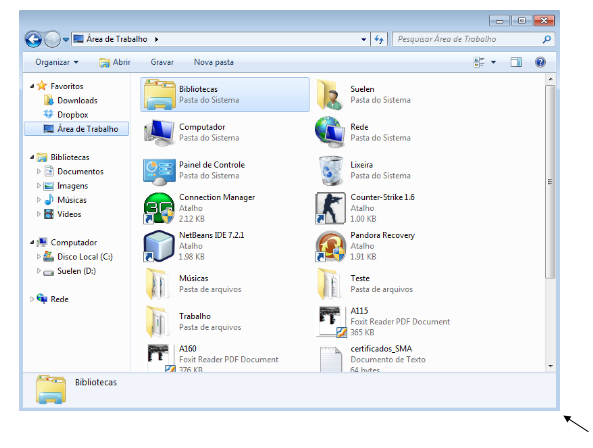
\includegraphics[scale=0.5]{Figures/red_janela}
		\caption{Leve o ponteiro do mouse até a área apontada pela seta como ilustrado acima}
		\label{fig:redimensionando janela}
		
	\end{figure}
	
	
	\section{Botões}
	
	
	\begin{figure}[!h]
			
\includegraphics[scale=0.5]{Figures/minimizar}
			\label{fig:min }
	\end{figure}
	
	\vspace{-1cm}{\bf Botão Minimizar}: reduz ou minimiza uma janela a um botão da barra de tarefas do Windows (seu programa se torna um ícone da barra de tarefas).
	
	\begin{figure}[!h]
		
\includegraphics[scale=0.5]{Figures/maximizar}
		\label{fig:max}
	\end{figure}
	
	\vspace{-1cm}{\bf Botão Maximizar}: aumenta ou maximiza uma janela (deixa a janela do tamanho da tela do computador).
	
	\begin{figure}[!h]
		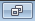
\includegraphics[scale=0.5]{Figures/restaurar}
		\label{fig:restaurar}
	\end{figure}
	
	\vspace{-1cm}{\bf Botão Restaurar}: restaura uma janela para o seu tamanho ou posição anterior.
	
	\begin{figure}[!h]
		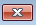
\includegraphics[scale=0.5]{Figures/fechar}
		\label{fig:fechar}
	\end{figure}
	
	\vspace{-1cm}{\bf Botão Fechar}: fecha um programa ou janela ativa. Caso um arquivo aberto não tenha sido salvo ou contenha alterações não salvas, você será solicitado a salvar ou não o arquivo antes de fechá-lo.
	
	
	\section{Movendo uma Janela}
	
	Para mover uma janela, leve o ponteiro do mouse até a barra de títulos. 	Segure o botão esquerdo do mouse e arraste a janela até a posição desejada.
	
	\begin{figure}[!h]
		\centering
		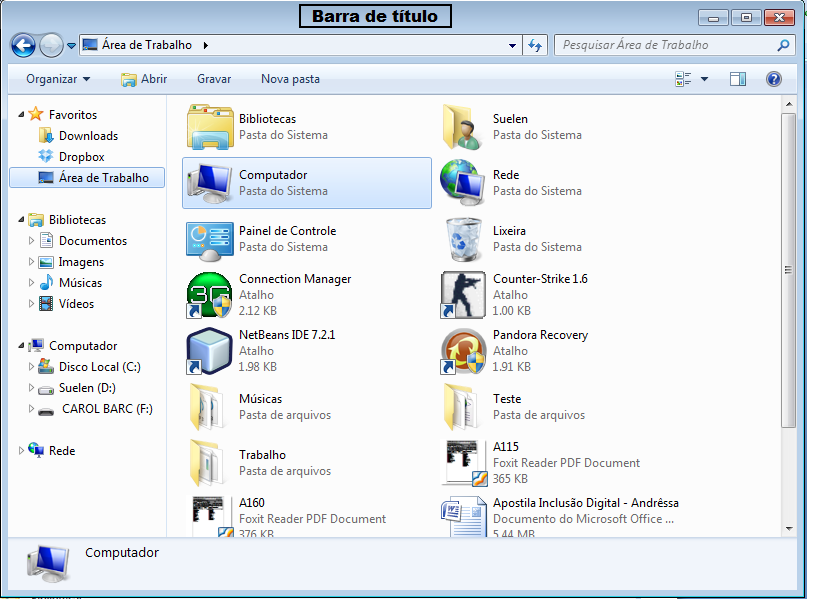
\includegraphics[scale=0.6]{Figures/mov_janela}
		\caption{Ilustração da localização da barra de título}
		\label{fig:movendo janela}
		
	\end{figure}
	
	\section{Pastas e Arquivos}
	
	É importante que mantenhamos os aplicativos e pastas de trabalho organizados. Em qualquer ambiente de trabalho, organização é fundamental para uma boa produtividade. Também é assim em um sistema operacional. O Windows já vem organizado de forma a facilitar essas rotinas. Contudo, nada impede que organizemos esse ambiente de acordo com nossas necessidades. Não se deve mexer, porém, nas pastas do sistema operacional, sob o risco de danificá-lo.

	A organização das pastas e arquivos pode ser observada através do Windows Explorer (ou Explorador). Como veremos mais adiante.
	
	\subsection{Criando uma pasta na área de trabalho}
	
	\begin{itemize}
		\item Em uma área vazia do desktop clique no botão direito do mouse. Escolha a opção{\bf Novo>Pasta}.
		\item Nomeie a pasta.
		\item Para abri-la, dê um clique duplo no botão esquerdo do mouse
		\item Podemos criar uma subpasta dentro da pasta principal utilizando o mesmo processo.
	\end{itemize}
	
		\begin{figure}[!h]
			\centering
			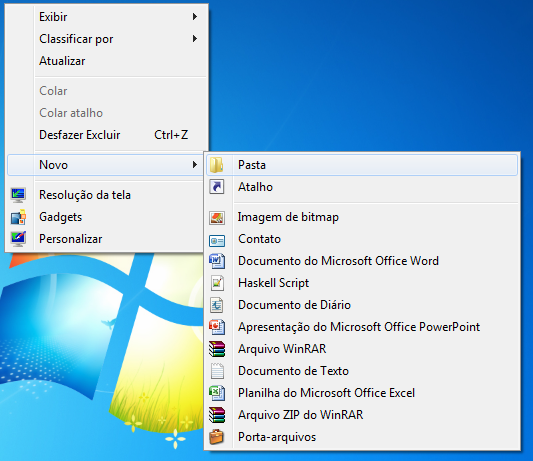
\includegraphics[scale=0.6]{Figures/cria_pasta}
			\caption{Criando pasta}
			\label{fig:criando pasta}
		\end{figure}
		
	\subsection{Windows Explorer}
	
		O Windows Explorer é uma ferramenta que auxilia na organização dos arquivos e pastas do disco rígido (HD).	
		
		Para acioná-lo, desça com a seta até o{\bf Menu iniciar>Todos os programas> Acessórios>Windows Explorer}.
	
		\begin{figure}[!h]
			\centering
			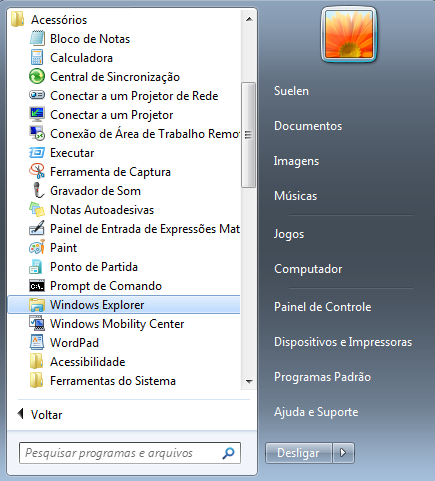
\includegraphics[scale=0.5]{Figures/explorer}
			\caption{Sequência para abrir o Windows Explorer}
			\label{fig:explorer}
		\end{figure}
		
			
			\begin{figure}[!h]
				\centering
				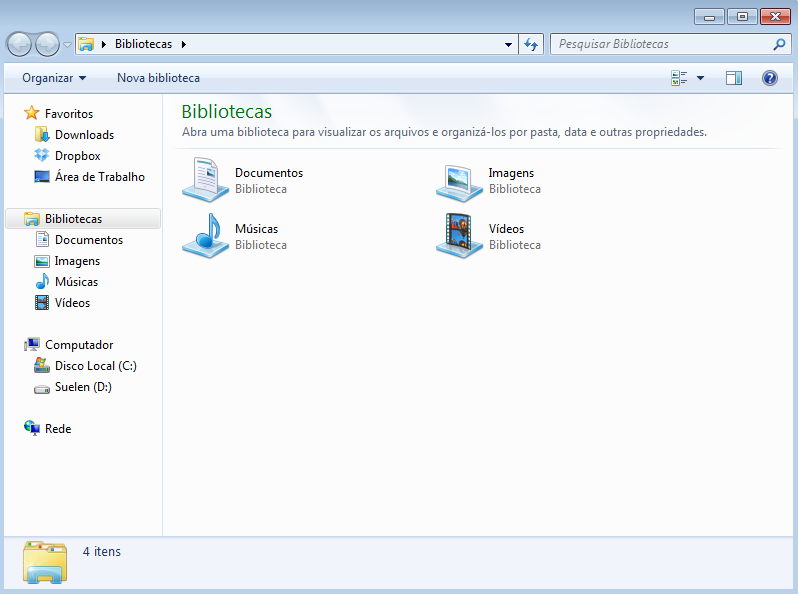
\includegraphics[scale=0.5]{Figures/explorer_pasta}
				\caption{Windows Explorer}
				\label{fig:explorer_p}
			\end{figure}
			
		\newpage	
		\subsection{Criando pastas no Windows Explorer}
		
		\begin{itemize}
			\item Selecionar o ícone {\bf(D:)}: clicando uma vez sobre ele com o botão esquerdo do mouse.
			\item Clique sobre uma área vazia com o botão direito do mouse. Escolha a opção{\bf Novo$>$Pasta}.
			\item Digite o nome da pasta e tecle o botão {\bf Enter}.
		\end{itemize}
		
		\begin{figure}[!h]
			\centering
			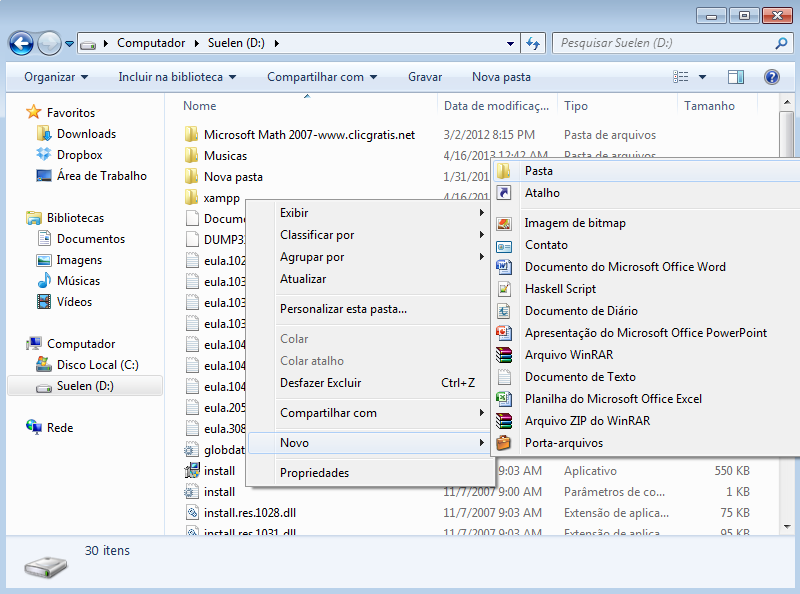
\includegraphics[scale=0.6]{Figures/passo1}
			\caption{Passo 1}
			\label{fig:passo1}
		\end{figure}
		
		
		\begin{figure}[!h]
			\centering
			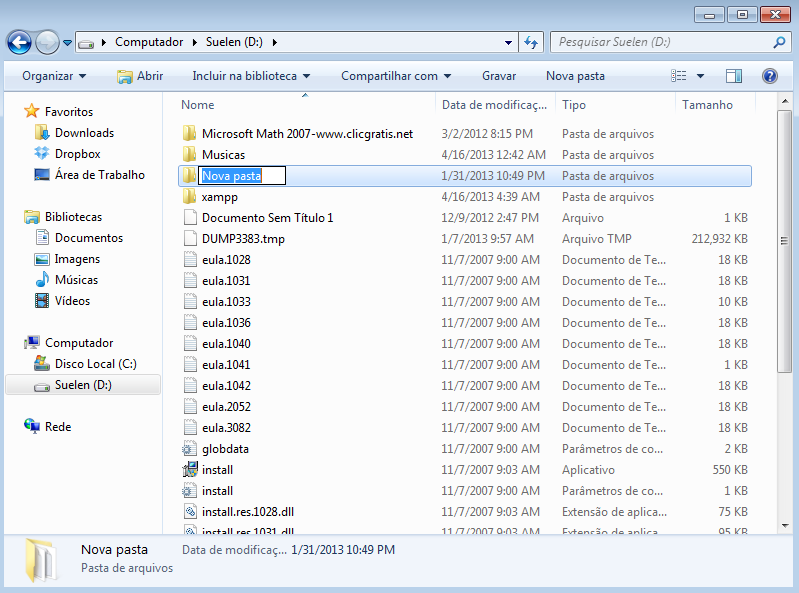
\includegraphics[scale=0.6]{Figures/passo2}
			\caption{Passo 2}
			\label{fig:passo2}
		\end{figure}
		
		\newpage
		\subsection{Copiando pastas (ou arquivos)}
		
		\begin{itemize}
			
			\item Selecionar o item a ser copiado clicando uma vez em cima do ícone com o botão esquerdo do mouse.
			\item Acionar o {\bf Copiar} (ou atalho {\bf Ctrl + C} - você aperta a tecla Ctrl do teclado e enquanto ela está acionada, aperta a letra {\bf C}, soltando ambas ao mesmo tempo).
			\item Selecionar a pasta que irá receber a cópia, clicar com o botão direito em cima do ícone.
			\item E clique na opção {\bf Colar}. Ou então podemos entrar na pasta e utilizar o comando ({\bf Ctrl + V} - você aperta a tecla {\bf Ctrl} do teclado e enquanto ela está acionada, aperta a letra {\bf V}, soltando ambas ao mesmo tempo)
		\end{itemize}
		
		\subsection{Movendo Pastas}
		
		\begin{itemize}
			\item Posicionar na pasta que será movida.
			\item Acessar o {\bf Recortar} (atalho {\bf Ctrl + X} - você aperta a tecla Ctrl do teclado e enquanto ela está acionada, aperta a letra {\bf X}, soltando ambas ao mesmo tempo).
			\item Selecionar o local de destino.
			\item Acessar o {\bf Colar}. Ou entrar na pasta e utilizar o atalho ({\bf Ctrl + V}).
		\end{itemize}
		
		\subsection{Renomeando Pastas}
		
		\begin{itemize}
			\item Selecionar a pasta, acessar o {\bf Menu Arquivo}(atalho {\bf Alt + A} - você aperta a tecla {\bf Alt} do teclado e enquanto ela está acionada, aperta a letra {\bf A}, soltando ambas ao mesmo tempo)>{\bf Renomear} (atalho F2) e digitar o novo nome.
		\end{itemize}
		
		\subsection{Apagando pastas e/ou arquivos}
		
		Basta selecionar a pasta e/ou arquivo, pressionar a tecla {\bf Delete} e confirmar pressionando o botão {\bf Sim}.
		
			\begin{figure}[!h]
				\centering
				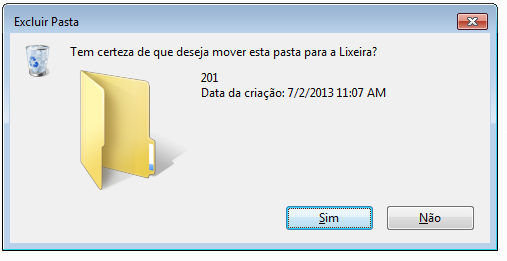
\includegraphics[scale=0.6]{Figures/delete}
				\caption{Janela de Confirmação de Exclusão}
				\label{fig:delete}
			\end{figure}
		
		\subsection{Renomeando Arquivos}
		
		\begin{itemize}
			\item Clicar com o botão direito em cima do ícone a ser renomeado.
			\item Clicar uma vez na opção {\bf Renomear}.
			\item Digitar o novo nome.
			\item Pressionar a tecla {\bf enter}.
		\end{itemize}
		
		\subsection{Localizando arquivos e pastas}
		
		\begin{itemize}
			\item Clique uma vez no ícone do Menu {\bf Iniciar}.
			
			\begin{figure}[!h]
				\centering
				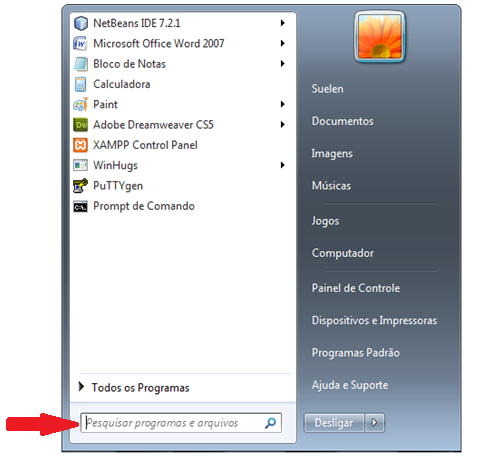
\includegraphics[scale=0.6]{Figures/localizar}
				\caption{Ilustração}
				\label{fig:localizar}
			\end{figure}
			
			\item  Basta digitar o nome do arquivo, pasta ou programa que deseja pesquisar na área apontada. Depois pressione a tecla {\bf enter}.
		\end{itemize}
		
		\subsection{Lixeira}
		
		É acessada através de um ícone na área de trabalho. Nela, são depositados os arquivos excluídos. Enquanto a Lixeira não for limpa, poderemos recuperar os arquivos apagados.
		
		\begin{figure}[!h]
			\centering
			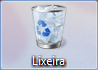
\includegraphics[scale=0.6]{Figures/lixeira}
			\caption{Ícone da lixeira}
			\label{fig:lixeira}
		\end{figure}
		\newpage
		Para remover definitivamente seu conteúdo, clique no botão do lado direito do mouse e escolha a opção {\bf Esvaziar Lixeira}.
		
		\begin{figure}[!h]
			\centering
			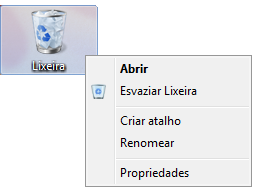
\includegraphics[scale=0.6]{Figures/esvaziar_lixeira}
			\caption{Esvaziar lixeira}
			\label{fig:esvaziar_lixeira}
		\end{figure}
		
		Para restaurar um arquivo, acesse a {\bf Lixeira}, escolha o arquivo a ser restaurado, clique nele com o botão direito do mouse, e em seguida clique na opção {\bf Restaurar}.
		
		\begin{figure}[!h]
			\centering
			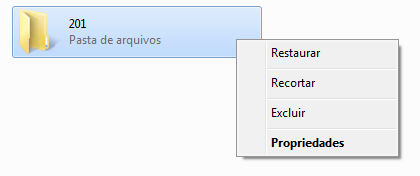
\includegraphics[scale=0.6]{Figures/restaurar_lixeira}
			\caption{Restaurar lixeira}
			\label{fig: restaurar_lixeira}
		\end{figure}
		
		\subsection{Exercícios}
		
		\begin{enumerate}
			
			\item Abra a pasta com o nome de {\bf Fotos} que se encontra na área de trabalho, clicando duas vezes sobre ela com o botão esquerdo do mouse. 
			
			
			\item Dentro desta pasta estão localizados dois arquivos de imagem com os seguintes nomes: {\bf Árvores} e {\bf Morangos}. Clique duas vezes sobre a imagem com o nome de {\bf Árvores}.
			
			\item Clique no botão {\bf Maximizar} que se localiza no canto superior direito da janela, do lado esquerdo do botão em vermelho (botão fechar). Note que a janela então expandirá para toda a tela.
			
			\item Agora clique no botão esquerdo do botão maximizar, o botão {\bf Minimizar}.
			
			\item Abra a segunda imagem com o nome de {\bf Morangos}. Feche então as duas janelas das imagens abertas.
			
			\item Agora minimize a janela da pasta {\bf Fotos} e então vá até a área de trabalho e crie uma pasta com o nome de {\bf Minha pasta}. 
			
			\item Vá até a pasta {\bf Fotos} e recorte os dois arquivos de imagens contidos nelas para a pasta {\bf Minha pasta}.
				
		\end{enumerate}
		
		
		\section{Aplicativos Diversos}
	
			Os programas de computador utilizados diretamente por pessoas comuns, como os editores de texto, são chamados de aplicativos.
			
			O Windows 7 vem com diversos aplicativos nativos e você pode instalar outros de acordo com suas necessidades. Para acessá-los vá até o {\bf Iniciar$>$Todos os programas} e escolher o aplicativo desejado. Alguns aplicativos úteis são:
			
			\begin{itemize}
				\item{
					{\bf Internet Explorer}: Usado para exibir páginas na Internet.
				\vspace{-1.2cm}{
				\begin{figure}[!h]
					
\includegraphics[scale=0.1]{Figures/ie}
					\label{fig:internet explorer}
				\end{figure}}
			}
			
			
			
			\item{
				{\bf Google Chrome}: Usado para exibir páginas na Internet.
				\vspace{-1.2cm}{
					\begin{figure}[!h]
						
\includegraphics[scale=0.1]{Figures/chrome}
						\label{fig:chrome}
					\end{figure}}
				}
				
				\item{
					{\bf Mozilla Firefox}: Usado para exibir páginas na Internet.
					\vspace{-1.2cm}{
						\begin{figure}[!h]
							
\includegraphics[scale=0.1]{Figures/firefox}
							\label{fig:firefox}
						\end{figure}}
					}
					
				
				\item{
					{\bf Windows Media Player}:reproduzir mídia digital, inclusive músicas, vídeos, CDs e DVDs.
					\vspace{-1.3cm}{
						\begin{figure}[!h]
							
\includegraphics[scale=1.2]{Figures/wmp}
							\label{fig:wmp}
						\end{figure}}
					}
			
			\end{itemize}
				
			Existem em outros diretórios, dezenas de aplicativos para diversas finalidades: Controle de sistemas, redes, teclado virtual, entre outros. Destacaremos a seguir os aplicativos usados com mais frequência.
			
			
			\begin{itemize}
				\item{
					{\bf Bloco de Notas}: cria e edita arquivos de textos utilizando formatação básica.
					\vspace{-1.3cm}{
						\begin{figure}[!h]
							
\includegraphics[scale=0.1]{Figures/bloco_notas}
							\label{fig:bloco_notas}
						\end{figure}}
					}
				
				\item{
					{\bf Calculadora}: executa tarefas aritméticas básicas com uma calculadora.
					\vspace{-1.3cm}{
						\begin{figure}[!h]
							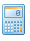
\includegraphics[scale=1]{Figures/calculadora}
							\label{fig:calculadora}
						\end{figure}}
					}
					
				\item{
					{\bf Paint}: cria e edita desenhos, além de exibir e editar fotos digitalizadas.
					\vspace{-1.5cm}{
						\begin{figure}[!h]
							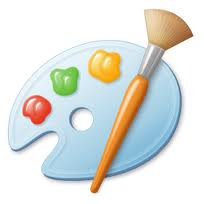
\includegraphics[scale=0.12]{Figures/paint}
							\label{fig:paint}
						\end{figure}}
					}
			\end{itemize}
			
			\subsection{Brincando com o paint}
			
			O Paint é um programa que compõe o grupo de acessórios do Windows 7. É um editor de imagens com diversos recursos para executar pequenos trabalhos de edição de imagens. Vamos conhecer as principais funções desse aplicativo e aprender a trabalhar com suas ferramentas.
			
			Na parte superior temos um Menu, uma Barra de ferramentas e uma Paleta de cores. Ao lado da Paleta de cores encontra-se um quadrado que indica a cor ativa no momento. Ao centro se localiza o plano de fundo, onde propriamente trabalhamos com o objeto a ser editado ou criado.
			
			\begin{figure}[!h]
				\centering
				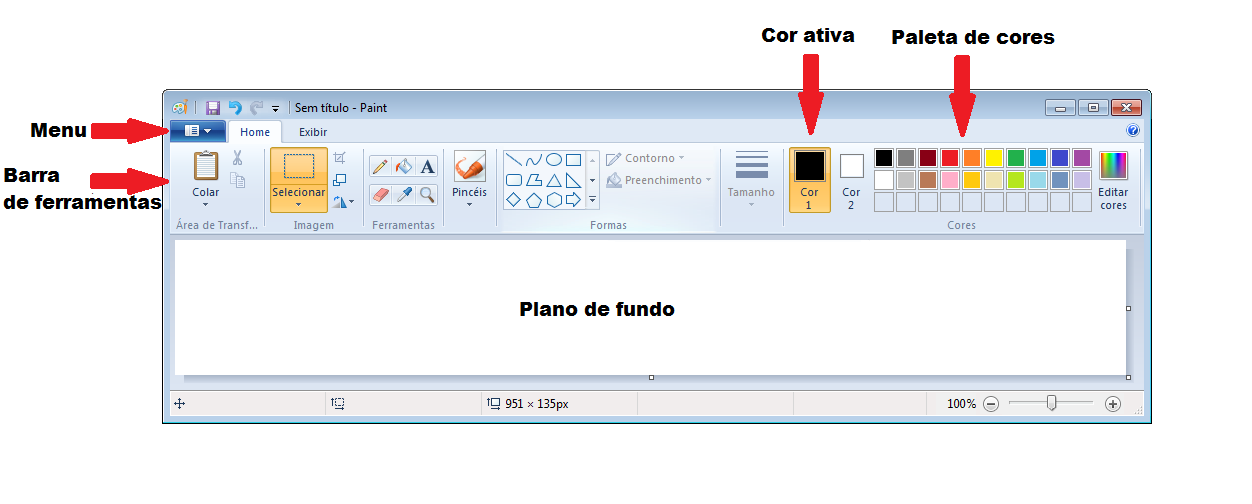
\includegraphics[scale=0.4]{Figures/paint1}
				\label{fig:paint1}
			\end{figure}
		
			\subsection{Recursos de desenho}	
			
			Os elementos fundamentais de trabalho do Paint residem na sua caixa de ferramentas. O desenho de linhas (retas ou curvas), de figuras prontas (círculo, retângulo, triângulo, etc.), a escrita de texto, o preenchimento de cores, selecionar, apagar, etc., são operações que passam pela ativação de um elemento da caixa de ferramentas. 
			
			Por baixo da caixa de ferramentas, existe um retângulo onde é possível visualizar outras opções relacionadas à ferramenta selecionada.
			
			
			\begin{figure}[!h]
				\centering
				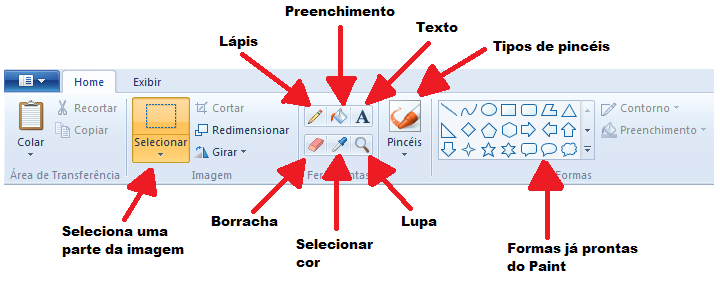
\includegraphics[scale=0.8]{Figures/paint2}
				\label{fig:paint2}
			\end{figure}
			
			\section{Recursos de desenho}
			
			Os elementos fundamentais de trabalho do Paint residem na sua caixa de ferramentas. O desenho de linhas (retas ou curvas), de figuras prontas (círculo, retângulo, triângulo, etc.), a escrita de texto, o preenchimento de cores, selecionar, apagar, etc., são operações que passam pela ativação de um elemento da caixa de ferramentas. Por baixo da caixa de ferramentas, existe um retângulo onde é possível visualizar outras opções relacionadas à ferramenta selecionada.
			
			
				
			\begin{figure}[!h]
				\centering
				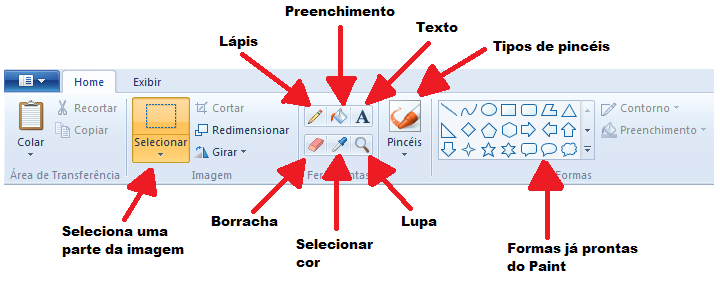
\includegraphics[scale=0.8]{Figures/paint3}
				\label{fig:paint3}
			\end{figure}
			
		
			\subsection{O Menu}
			
			Os arquivos criados pelo Paint por padrão são salvos como bitmap (.bmp). Porém podem ser salvos também em JPEG (.jpg), GIF (.gif), PNG (.png) entre outros.
			
			No Menu, encontre o seguinte ícone:
			
			\begin{figure}[!h]
				\centering
				
\includegraphics[scale=0.8]{Figures/iconep}
				\label{fig:paintp}
			\end{figure}
			
			Uma janela abrirá com as seguintes opções:
			
			\begin{itemize}
				\item {\bf Nova} – permite criar um novo arquivo;
				
				\item {\bf Abrir} – permite abrir um arquivo existente;
				
				\item {\bf Salvar} – permite gravar o arquivo aberto;
				
				\item {\bf Salvar como} – permite gravar o arquivo aberto com outro nome, formato ou em outro local;
				
				\item {\bf Imprimir} – Imprime o arquivo que está sendo editado pelo Paint;
				
				\item {\bf Definir como plano de fundo da área de trabalho} – Define o arquivo que está sendo editado pelo Paint como imagem de fundo da área de trabalho.
				
				\item {\bf Sair} – permite fechar o aplicativo.
			\end{itemize}
			\bigskip
			\begin{figure}[!h]
				\centering
				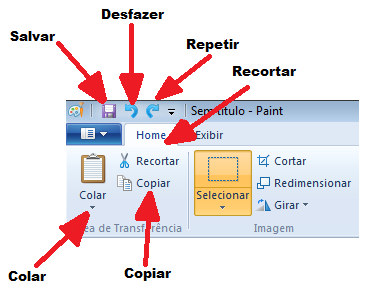
\includegraphics[scale=0.8]{Figures/paint4}
				\label{fig:paint4}
				\caption{Formas de edição no paint}
			\end{figure}
			
			\begin{itemize}
				\item {\bf Desfazer} – anula a última ação;
				
				\item {\bf Repetir} – repete a ação anulada;
				
				\item {\bf Recortar} – corta a seleção para a Área de Transferência;
				
				\item {\bf Copiar} – copia a seleção para a Área de Transferência;
				
				\item {\bf Colar} – insere o conteúdo da Área de Transferência;
				
				\item {\bf Salvar} – salva o arquivo que está sendo editado.
			\end{itemize}
			
			\subsection{Calculadora}

			A calculadora do Windows 7 é acionada através do caminho: {\bf Iniciar $>$ Todos os programas $>$ Acessórios $>$ Calculadora}. Pode ser utilizada através do mouse ou com o uso do teclado numérico.
			
			No item Exibir, você pode alternar a visualização da calculadora entre Padrão e Científica, Programador e Estatística.	
			
			\begin{figure}[!h]
				\centering
				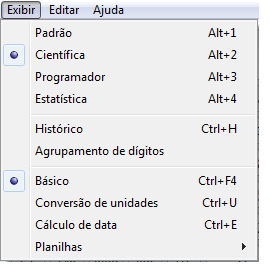
\includegraphics[scale=0.8]{Figures/calc1}
				\label{fig:calc1}
				\caption{Exibir}
			\end{figure}
			
			\begin{figure}[!h]
				\centering
				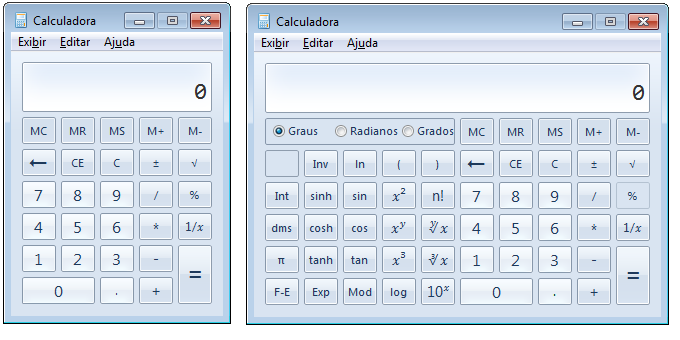
\includegraphics[scale=0.8]{Figures/calc2}
				\label{fig:calc2}
				\caption{Calculadoras Padrão e Científica, respectivamente}
			\end{figure}
			
		\subsection{Exercícios}
			
		\begin{enumerate}
			\item Abra o aplicativo referente à calculadora ({\bf Iniciar $>$ Todos os programas $>$ Acessórios $>$ Calculadora}). Clique no número 6, multiplique por 64, subtraia 20 e divida por 7.
		\end{enumerate}
			
	\section{Microsoft Office 2007}
	
	\subsection{Apresentação}
	
	O Word 2007 faz parte do pacote de produtividade Microsoft® Office System de 2007, que sucedeu ao Office 2003.

	Seu principal objetivo é a criação e edição de textos, porém existem ainda várias outras ferramentas muito úteis para o usuário.
		
	\subsection{Executando o Programa}
	
	\begin{itemize}
		\item Dê um clique no botão \textbf {Iniciar};

		\item Posicione a seta do mouse sobre \textbf{Todos os Programas};
		
		\item Posicione a seta do mouse sobre \textbf{Microsoft Office};
		
		\item Posicione a seta do mouse e dê um clique sobre \textbf{Microsoft Office Word 2007}.
		
		
	\end{itemize}
	
	\begin{figure}[!h]
		\centering
		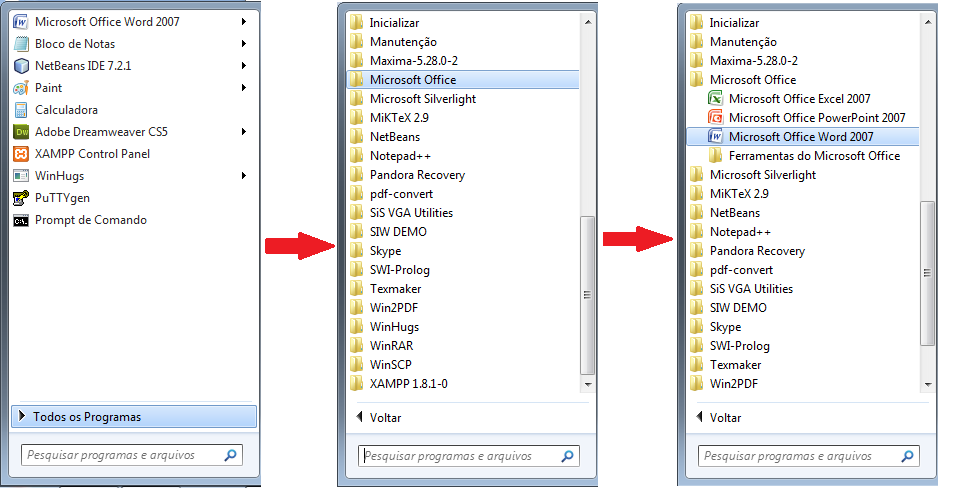
\includegraphics[scale=0.5]{Figures/office1}
		\label{fig:office1}
		\caption{Abrindo o Microsoft Office 2007}
	\end{figure}
			
	\newpage		
	\subsection{Ambiente de Trabalho}
		
		\begin{figure}[!h]
			\centering
			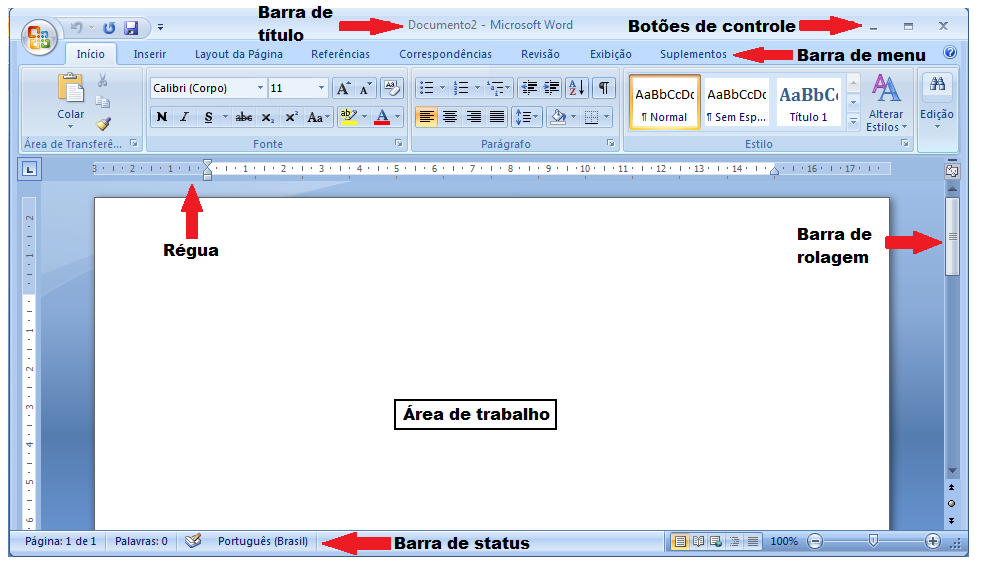
\includegraphics[scale=0.5]{Figures/office2}
			\label{fig:office2}
			\caption{Conhecendo o Microsoft Office 2007}
		\end{figure}
				
	\subsection{Criando Texto}

		
		\begin{itemize}
			\item Clique na área de trabalho;
			
			\item Digite o texto a seguir:
		\end{itemize}
		
		
		{\textbf{\hspace{5cm} Para refletir}}
		
		"A melhor de todas as coisas é aprender. O dinheiro pode ser perdido ou roubado, a saúde e força podem falhar, mas o que você dedicou à sua mente é seu para sempre." (\emph{Louis L'Amour}).
		
		
		
	\subsection{Editando Texto}
		
		\begin{itemize}
			\item Selecione o título com o mouse;
			
			\item Altere as características da fonte como desejar;
			
			\item Agora vamos alterar as características do texto, basta seguir os passos anteriores;
			
			\item Não se esqueça de alinhar seu texto da melhor maneira possível.
		\end{itemize}
		

	\subsection{Salvando o documento}
	
	\begin{itemize}
		\item Clique no menu \textbf{Office}:
		
		\begin{figure}[!h]
			\centering
			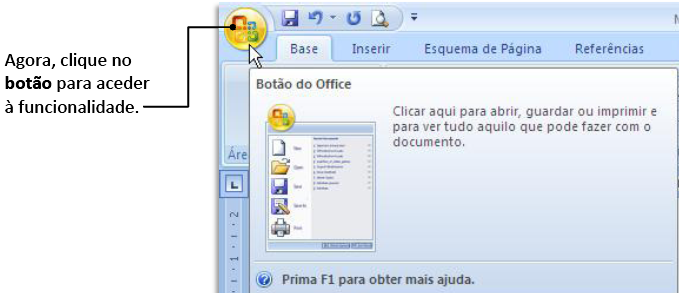
\includegraphics[scale=0.5]{Figures/office3}
			\label{fig:office3}
			\caption{Salvando um documento}
		\end{figure}
		
		\item Clique no botão \textbf{Salvar}:
		
		\begin{figure}[!h]
			\centering
			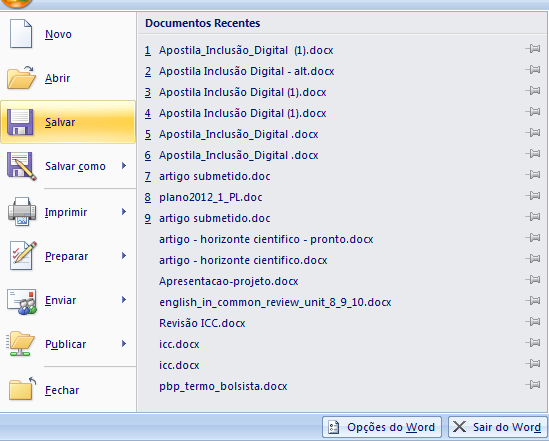
\includegraphics[scale=0.5]{Figures/office4}
			\label{fig:office4}
		\end{figure}
		
		
		\item Encontre o local desejado para guardar seu documento, dê o nome desejado e clique em \textbf{Salvar};
		
		\item Pronto, agora seu arquivo está guardado em seu computador. Poderá utilizar e alterá-lo sempre que desejar
		
	\end{itemize}
				
	\subsection{Criando um novo Documento}
	
	\begin{itemize}
		
		\item Clique no \textbf{botão Office} e escolha opção \textbf {Novo};

		\item A janela a seguir abrirá:
		
		
		\begin{figure}[!h]
			\centering
			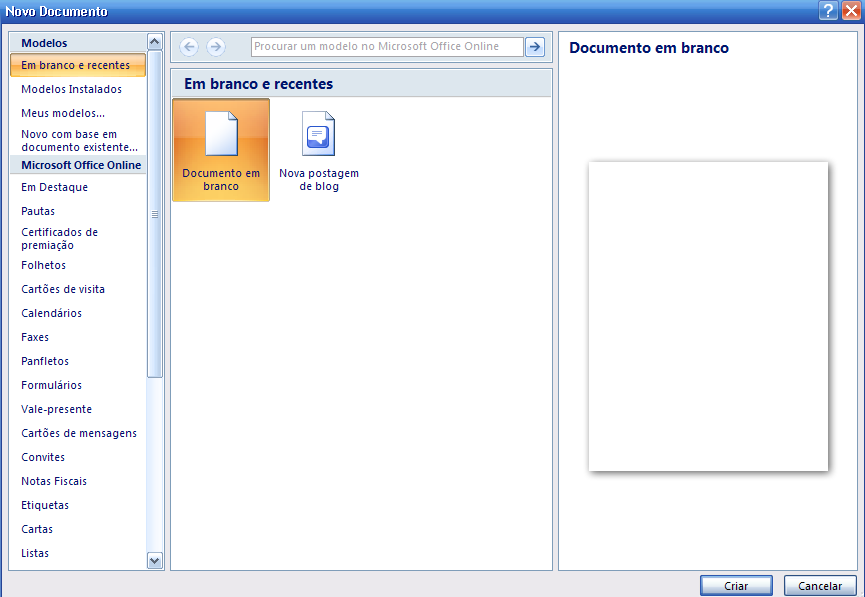
\includegraphics[scale=0.5]{Figures/office5}
			\label{fig:office5}
			\caption{Criando um novo documento}
		\end{figure}
		
		\item Clique em \textbf{Criar};

		\item Novo documento foi aberto e está pronto para ser utilizado;
		
		
	\end{itemize}
	\newpage
	\subsection{Abrindo um documento}
	
		\begin{itemize}
			
		\item Abra o Word como foi explicado anteriormente;

		\item Clique no botão \textbf{Office} e escolha a opção \textbf{Abrir};
		
		\item A seguinte janela abrirá:
		
		\begin{figure}[!h]
			\centering
			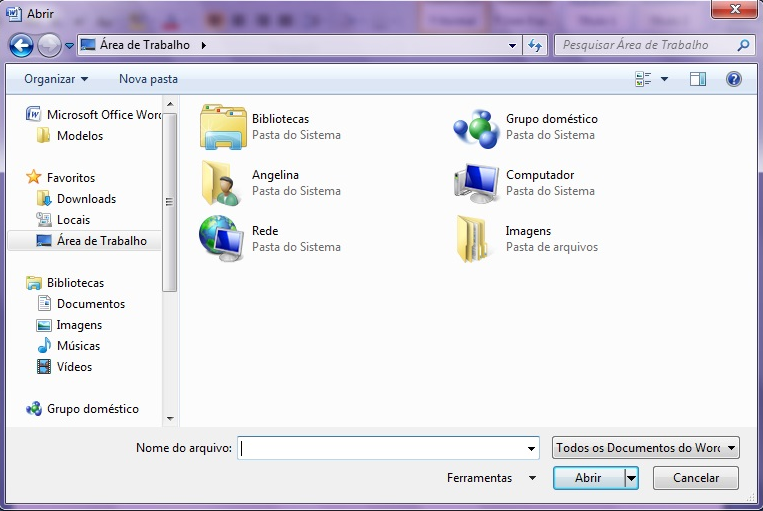
\includegraphics[scale=0.5]{Figures/office6}
			\label{fig:office6}
			\caption{Janela para abrir documentos}
		\end{figure}

		\item Procure o local onde se encontra o arquivo desejado. Clique nele e depois em \textbf{Abrir};
		
		\item Para praticar, formate novamente seu texto, alternando fonte, tamanho, cor, dentre outros.
			
		\end{itemize}	
		
	\subsection{Desfazendo e Refazendo uma Ação}
	
	
	\begin{figure}[!h]
		\centering
		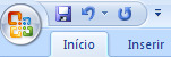
\includegraphics[scale=1]{Figures/office7}
		\label{fig:office7}
		\caption{Botões desfazer e refazer}
	\end{figure}
	
	\icon{Figures/desfazer} \textbf{Desfazer} - caso você cometa algum erro, ou deseje desfazer uma ação, para voltar ao que era antes, basta clicar no botão desfazer, ele desfaz a última ação que você fez no Microsoft Word. Outra opção para desfazer o que foi digitado é utilizar o atalho do teclado \textbf{Ctrl + Z};\\
	
	\icon{Figures/refazer} \textbf{Refazer} - o botão refazer só é acionado se você utilizar o botão desfazer, o refazer refaz novamente a ação que você desfez através do botão desfazer, seja um erro ou qualquer outra ação.
	
	Para treinarmos a função desses botões siga os passos abaixo:
	
	\begin{enumerate}
		\item Dê um clique no botão \icon{Figures/novo} \textbf{Novo} para abrir um novo documento;
		
		\item Escolha o tamanho de fonte \textbf{20};
		
		\item  Digite a palavra: \textbf{Treinamento!}
		
		
		\item Selecione a palavra que você acabou de digitar e em seguida pressione a tecla \textbf{Delete};
		
		\item Dê um clique no botão \icon{Figures/desfazer} Desfazer. Observe que a palavra digitada retornou  a tela.                                                               
		
		\item Agora dê um clique no botão \icon{Figures/refazer} Refazer.
	\end{enumerate}

	Observe que a palavra digitada foi apagada novamente, pois foi refeita sua última ação, a qual foi apagar a palavra.            
	
	
	\subsection{Recortar, Copiar, Colar}
	
	\icon{Figures/recortar} \textbf{Recortar} - Você pode recortar qualquer coisa que estiver selecionada e depois colá-la em outro lugar. (Quando você recorta algo, você retira de um local e pode colocar em outro). Outra opção para recortar o que foi digitado é utilizar o atalho do teclado \textbf{Ctrl + X}; 
	
	\icon{Figures/copiar} \textbf{Copiar} - O botão copiar serve para você copiar o que estiver selecionado e depois colá-lo em outro lugar. (Quando você utiliza a opção copiar, você está duplicando o que copiou). Outra opção para copiar o que foi digitado é utilizar o atalho do teclado \textbf{Ctrl + C}; 
	
	\icon{Figures/colar} \textbf{Colar} - O botão colar só pode ser utilizado depois de você ter \textbf{recortado} ou \textbf{copiado} algo. (O item recortado ou copiado será colado onde o cursor estiver posicionado).
	
	\subsection{Treinamento}
		
		\begin{enumerate}
			\item Escolha o \textbf{Tamanho de Fonte 29};

			\item Digite em letras Maiúsculas: \textbf{TREINAMENTO};
			
			\item Selecione o que você digitou;
			
			\item Dê um clique no botão \icon{Figures/copiar} \textbf{Copiar} ou utilize o atalho \textbf{Ctrl + C}; 
			
			\item Retire a Seleção clicando em algum lugar da página de texto;
			
			\item Posicione o cursor no final da linha e pressione \textbf{Enter};
			
			\item Dê um clique no botão \icon{Figures/colar} \textbf{Colar} ou utilize o atalho \textbf{Ctrl + V}; 
			
			\item Dê novamente um clique no botão \icon{Figures/colar}  \textbf{Colar} (Observe que você duplicou a palavra);
			
			\item Pressione a tecla \textbf{Enter};
			
			\item Escolha o tamanho de fonte \textbf{35};
			
			\item Digite em letras maiúsculas: \textbf{TREINAMENTO};
			
			\item Pressione \textbf{Enter};
			
			\item Digite em letras maiúsculas: \textbf{INFORMÁTICA};
			
			\item Pressione \textbf{Enter};
			
			\item Digite em letras maiúsculas: \textbf{NEP – Laguna};
			
			\item Pressione \textbf{Enter};
			
			\item Selecione a linha \textbf{INFORMÁTICA}; 
			
			\item Dê um clique no botão  \icon{Figures/recortar} \textbf{Recortar} - ou utilize o atalho \textbf{Ctrl + X};
			
			\item Posicione o cursor no final da linha \textbf{NEP – Laguna};
			
			\item Pressione \textbf{Enter};
			
			\item Dê um clique no botão \icon{Figures/colar} \textbf{Colar} (Observe que as palavras recortadas anteriormente aparecem no local onde você deixou o cursor).
			
			\item Agora \textbf{Salve} as Alterações em sua pasta com o nome de \textbf{Exercício 04}.   
		\end{enumerate}
	
	\subsection{Exercícios}
	
	\begin{enumerate}
		\item Para praticar os conhecimentos adquiridos e sua digitação, dê um clique no botão \icon{Figures/novo}
		 \textbf{Novo} para abrir um novo documento;

		\item Digite o seguinte texto para praticar acentuação, não esqueça os marcadores.
		
		\begin{enumerate}
			\item Palavras com Acento Agudo:
			Pó, Café, Boné, Saúde, Água, Vídeo, Vovó.
			
			\item Palavras com Acento Circunflexo: Vê, Têm, Silêncio, Eletrônica, Vovô, Crochê, Crê.
			
			\item Palavras com Cedilha: Laço, Braço, Abraço, Berço, Força, Espaço, Faço.
			
			\item Palavras com Til: Coração, Emoção, Avião, Tentação, Tubarão, Aplicação
		\end{enumerate}	
			
			
		\item Altere o texto dando-lhe uma boa aparência. Crie um título.     
	\end{enumerate}
			
	\subsection{Inserindo uma Imagem no documento}
		
		O Microsoft Word oferece o recurso de se adicionar ao documento imagens que estejam no computador.
			
	\begin{enumerate}
	
		
		\item Dê um clique no botão \icon{Figures/novo} \textbf{Novo} para abrir um novo documento;
		
		\item Dê um clique no \textbf{Menu Inserir}, em seguida no ícone \icon{Figures/imagem};
		
		\item Observe que abrirá a janela \textbf{Inserir Imagem}. Esta janela será utilizada para encontrar a imagem desejada, que está no computador;
		
		\item Clique em \icon{Figures/desk} e em seguida selecione a imagem \textbf{Tulipa} e clique em \textbf{Inserir}, ou simplesmente dê um duplo clique na imagem desejada;
		
		\item Dê UM clique sobre a figura;
		\begin{figure}[!h]
			\centering
			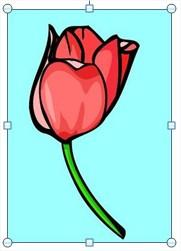
\includegraphics[scale=1]{Figures/tulipa}
			\label{fig:tulipa}
			\caption{Figura da Tulipa}
		\end{figure}
		
		
		
		\item Observe que a figura ficou cercada por 8 pontos. Eles servem para \textbf{Aumentar} ou \textbf{Diminuir} a imagem, sempre que você desejar alterar o tamanho posicione a seta sobre um dos 4 cantos de modo que apareça uma seta dupla (você deve alterar o tamanho pelos cantos para que a imagem não fique achatada);
		
		\item Agora tente alterar o tamanho de sua Imagem. Feito isso clique novamente sobre a mesma e pressione a tecla \textbf{DELETE}.
		
	\end{enumerate}
	
	\subsection{Treinando a Inserção de Imagens}
	
	\begin{enumerate}
		
		
		
			\item Escolha o tamanho de fonte \textbf{14};
			
			\item Digite o texto abaixo seguindo as formatações e inserindo imagens que você goste e estejam na Área de trabalho (desktop):
			
	\end{enumerate}
		\newpage
		
		{\centering \textbf{AMOR}\\
			
			Amor é fogo que arde sem se ver;
			\begin{figure}[!h]
				\centering
				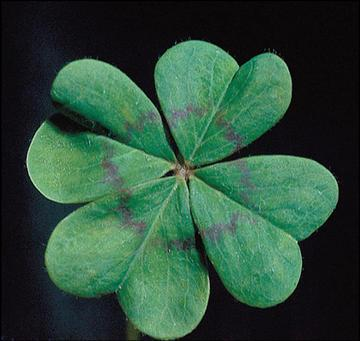
\includegraphics[scale=0.3]{Figures/trevo}

			\end{figure}
			
			É ferida que dói e não se sente;
			\begin{figure}[!h]
				\centering
				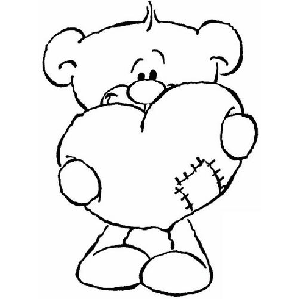
\includegraphics[scale=0.3]{Figures/urso}
			\end{figure}
			
			É um contentamento descontente;  
			
			\begin{figure}[!h]
				\centering
				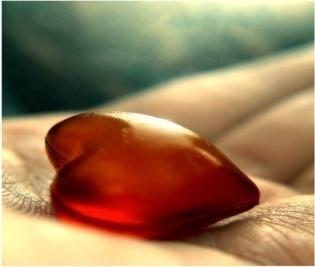
\includegraphics[scale=0.6]{Figures/coracao}
			\end{figure}
			É dor que desatina sem doer.
			
			}
			\bigskip
	
		3. Agora, \textbf{Salve} em sua pasta com o nome de \textbf{Exercício 07}.
		
		\subsection{Fazendo um Cartão}
		
		\begin{enumerate}
			\item Clique com o botão esquerdo do mouse na figura 

			\item Clique em \textbf{Ferramentas de Imagens} na barra acima do texto.
			
			\begin{figure}[!h]
				\centering
				\includegraphics[scale=0.6]{Figures/office8}
				
			\end{figure}
			\newpage
			\item Clique em \textbf{Quebra Automática de Texto};
			
			\begin{figure}[!h]
				\centering
				\includegraphics[scale=0.5]{Figures/office9}
				
			\end{figure}
			
			\item Clique em \textbf{Atrás do Texto}. Ao Fazer isso, você enviou a imagem para trás do texto que vocês estão escrevendo. O que significa isso? Significa que agora vocês podem escrever por cima da imagem que vocês quiserem, mudar o tamanho e outras propriedades da imagem.
			
			\begin{figure}[!h]
				\centering
				\includegraphics[scale=0.5]{Figures/office10}
				
			\end{figure}
			
			\item Esticar a figura, aumentar, diminuir;

			\item Clique na figura e, em seguida, \textbf{Ferramenta de Imagens};
			
			\item Clique em \textbf{Brilho} e mude-o para verificar o que acontece com a figura;
			
			\item Clique em \textbf{Contraste} e modifique-o também.
			
			
			\begin{figure}[!htbp]
				\centering
				\begin{minipage}[b]{0.4\textwidth}
					\includegraphics[width=\textwidth]{Figures/office11}
					\caption{Brilho}
				\end{minipage}
				\hfill
				\begin{minipage}[b]{0.4\textwidth}
					\includegraphics[width=\textwidth]{Figures/office12}
					\caption{Contraste}
				\end{minipage}
			\end{figure}
			
			\item Para finalizar, siga o mesmo procedimento anterior (\textbf{Clicar na Figura $>$ Ferramentas de Imagens $>$ Quebra automática de texto $>$ Atrás do Texto}) e depois clique em cortar.
			
			\newpage
			
			\item  Perceba que apareceram umas bordas pretas na imagem como a seguir:
			\begin{figure}[!htbp]
				\centering
				\begin{minipage}[b]{0.9\textwidth}
					\includegraphics[width=\textwidth]{Figures/office13}
					
				\end{minipage}
				\hfill
				\begin{minipage}[b]{0.9\textwidth}
					\includegraphics[width=\textwidth]{Figures/office14}
					
				\end{minipage}
			\end{figure}
			
			
		\end{enumerate}
		
		Se você mexer em uma das bordas, perceba que a figura diminui. Um exemplo de utilidade dessa ferramenta é a seguinte: Suponhamos que alguém indesejado apareça em sua foto, basta usar essa ferramenta para cortar \footnote{Função também disponível no programa Paint} essa pessoa ou imagem indesejada da foto .
		
		\section{Internet}
		
		\subsection{O que é Internet}
		
		A Internet é uma gigantesca rede mundial de computadores espalhados por todo o planeta e interligados através de linhas comuns de telefone ou outros meios de telecomunicação. Ela tem o objetivo de estabelecer a troca de informação e serviços, unindo usuários particulares, órgãos governamentais, grupos de pesquisa, bibliotecas e grandes empresas. 

		A Internet surgiu de um projeto militar do governo americano no início da década de 50, mas se expandiu e já conta com 1,73 bilhões de usuários, sendo 60 milhões de brasileiros.
		
		\subsection{Conceitos Básicos da Internet}
		
		\textbf{Site}
		
		É uma coleção de páginas web, isto é, de documentos acessíveis através da web, na internet. Os sites da Internet, em geral, podem ter os seguintes propósitos:

		\textbf{Institucional}: muitas empresas usam seus sites como ponto de contato entre uma instituição e seus clientes ou fornecedores. Instituições comerciais podem usar seus websites para comércio eletrônico ou até para recrutamento. 
		
		Ex.: http://www.ufu.br/ (Site da Faculdade de Engenharia Mecânica da UFU);
		
		
		\textbf{Informações}: veículos de comunicação como jornais, revistas, agências de notícias ou mesmos jornalistas independentes utilizam a Internet para veicular notícias, por meio de seus sites. 
		
		Ex.: \url{http://www.joelmirbeting.com.br}/(blog do jornalista especialista em economia Joelmir Beting);
		
		
		\textbf{Aplicações}: existem sites cujo conteúdo contém processadores de texto, planilhas eletrônicas, editores de imagem, softwares de correio eletrônico, agendas, etc. 
		
		Ex.: \url{http://docs.google.com} (exemplo de site que apresenta as ferramentas do desktop);
		
		
		\textbf{Comunitário}: são os sites que servem para a comunicação de usuários com outros usuários da rede. Nesta categoria se encontram os chats, fóruns e sites de relacionamento. 
		
		Ex.: \url{http://www.facebook.com/} (site de relacionamentos);
		
		
		\textbf{Portais}: são chamados de "portais" os sites que congregam conteúdos de diversos tipos entre os demais tipos, geralmente fornecidos por uma mesma empresa. Recebem esse nome por congregarem a grande maioria dos serviços da Internet num mesmo local. 
		
		Ex.: \url{http://g1.globo.com/} (portal de notícias da globo).
				
	
\end{document}
